In this section, we answer the question posed at the end of Section
\ref{sec:energy_detector} by defining $\kuse$, the number of useful signal components. We
show that $\kuse$ is dependent on $\delta$ and the desired false alarm rate $P_F$. We
provide some intuition behind our definition by discussing how the conditional
distributions of the energy detector's test statistic shift when adding additional
components. If an additional signal component further separates the conditional
distributions, it is one of the $\kuse$ components in detection; otherwise, including that
component would degrade detector performance. Of particular importance, $\kuse$ may be
less than the inherent dimension, $k$, of the observed data, even when $\delta_i\neq0$.

\subsection{Definition and Computation of $\kuse$}

We define the number of useful detection components at a false alarm rate $P_F$ as the
solution to the following optimization problem
\beq\label{eq:opt_prob}
\kuse = \argmax_{d\in\{1,\dots,k\}} P_{D_{\text{energy}}}(P_F,d)
\eeq 
where $P_{D_{\text{energy}}}(P_F,d)$ is defined in (\ref{eq:roc_energy}). This is the
optimal number of components to include in an energy detector in (\ref{eq:the_detector})
to maximize detector performance. Using exactly $\kuse$ components includes all components
that improve detection ability and excludes all components that degrade detection ability.

To determine $\kuse$, we propose the greedy ``algorithm'' in Figure \ref{algo:kuse}. The
algorithm relies on the fact that the components of $\delta$ are ordered
(i.e. $|\delta_1|\geq\dots|\delta_k|$). It adds one component at a time and searches for
the last component that resulted in an increase in detection ability. This algorithm
relies on knowledge of $\delta$ and so by definition $\kuse$ is an oracle quantity.
Therefore, a realizable detector using exactly $\kuse$ components is currently beyond
reach. Estimating $\kuse$ is a topic for future work and may involve placing a prior
distribution on the test vector. In Section \ref{sec:msd}, we discuss using the effective
number of subspace components, $\keff$, as an estimate for $\kuse$.

%\begin{figure}
% \hrulefill
%  \begin{algorithmic}[1]


\begin{algorithm}
  \KwIn{$P_F$, $\delta$ }

  Compute $P_D(P_F,1)$ from (\ref{eq:roc_energy})

  \For{$h=2,\dots,k$} {

    Compute $P_D(P_F,h)$ from (\ref{eq:roc_energy})

    \If{$P_D(P_F,h) < P_D(P_F,h-1)$}{

      $\kuse= h-1$

      \textbf{Return:} $\kuse$
    }
  }
  $\kuse = k$

  \KwOut{$\kuse$ }
  \caption{Algorithm to determine $\kuse$. This is computable in an oracle setting\\
    where $\delta$ is known.}  
  \label{algo:kuse}
\end{algorithm}

\subsection{Discussion of Test Statistic Distributions}

In order to provide intuition behind the definition of $\kuse$, we examine the conditional
distribution of the test statistic in (\ref{eq:the_detector}):
\beq\label{eq:d_distrs}\ba
& \Lambda_d(w)\,|\,H_0 \sim\chi^2_d,\\
& \Lambda_d(w)\,|\,H_1 \sim\chi^2_d(\lambda_d)\\
\ea\eeq
where
\beq\label{eq:nc_param}
\lambda_d = \sum_{i=1}^d \delta_i^2.
\eeq
Clearly, both distributions and the non-centrality parameter depend on $d$. Therefore, a
closed form expression for $\kuse$ is not possible and we rely on the greedy algorithm
in Figure \ref{algo:kuse}. Adding an additional component presents a tradeoff between
adding $\delta_i^2$ to the non-centrality parameter and adding 1 to the degrees of
freedom in the c.d.f's in (\ref{eq:d_distrs}).

This tradeoff becomes more evident when using (\ref{eq:roc_energy}) to rewrite the
optimization problem in (\ref{eq:opt_prob}) as
\beq\label{eq:simple_opt}
\kuse = \argmin_{d\in\{1,\dots,k\}}
Q_{\chi_{d}^2(\lambda_d)}\left(Q^{-1}_{\chi^2_{d}}\left(1-P_F\right)\right). 
\eeq

By fixing the signal distribution $Q_{\chi^2_d(\lambda_d)}$, solving (\ref{eq:simple_opt}) is
equivalent to minimizing $Q^{-1}_{\chi^2_{d}}\left(1-P_F\right)$, which is achieved when
$d=1$. This minimizes the variance contribution from the noise distribution. However, by
fixing the noise distribution $Q_{\chi^2_d}$, solving (\ref{eq:simple_opt}) is equivalent
to minimizing $Q_{\chi_{d}^2(\lambda_d)}\left(\cdot\right)$, which is achieved when
$d=k$. This maximizes the variance contribution from the signal distribution. The solution
to (\ref{eq:simple_opt}) is dependent on how much each additional component contributes to
the overall non-centrality parameter. If the contribution is large enough, the added
variance in the noise distribution from the extra degree of freedom is overcome by the
distribution shift induced by the increase in non-centrality parameter.

To illustrate how the conditional distributions shift when adding components to the energy
detector, Figure \ref{fig:distributions} plots the distributions of $\Lambda_d(w)|H_0$ and
$\Lambda_d(w)|H_1$ for three choices of $d$ and $\lambda_d$. Figure \ref{fig:small} sets
$d=1$ and $\lambda_d=2$ and is used as a baseline. Figure \ref{fig:med} increases the
number of components to $d=2$ while keeping the non-centrality parameter fixed at
$\lambda_d=2$. The added component increases the noise variance by 2. However, as there is
no increase in the non-centrality parameter, the signal variance also increases by
2. Thus, the signal-to-noise ratio is effectively decreased. Therefore, the second
component causes the conditional distributions to become more similar and thus degrades
detector performance; therefore, $\kuse=1$. Figure \ref{fig:big} keeps the number of
components at $d=2$ but increases the non-centrality parameter to $\lambda_d=3$. In this
setting, the increase in non-centrality parameter increases the signal variance, which
overcomes the resulting increase in noise variance. The second component further separates
the conditional distributions and improves detection performance; therefore,
$\kuse=2$. Figure \ref{fig:dist_roc} plots the corresponding ROC curves for the three
choices of parameters in Figure \ref{fig:distributions}. When adding a component causes
the conditional distributions to better separate as in Figure \ref{fig:big}, the resulting
ROC curve shows an improvement in detection. \textit{For an additional component to be one
  of the $\kuse$ components, the resulting increase in noise variance must be overcome by
  a sufficiently large enough increase in non-centrality parameter.}

\begin{figure}[t]
\centering
\subfigure[$d=1$, $\lambda_d=2$]{
  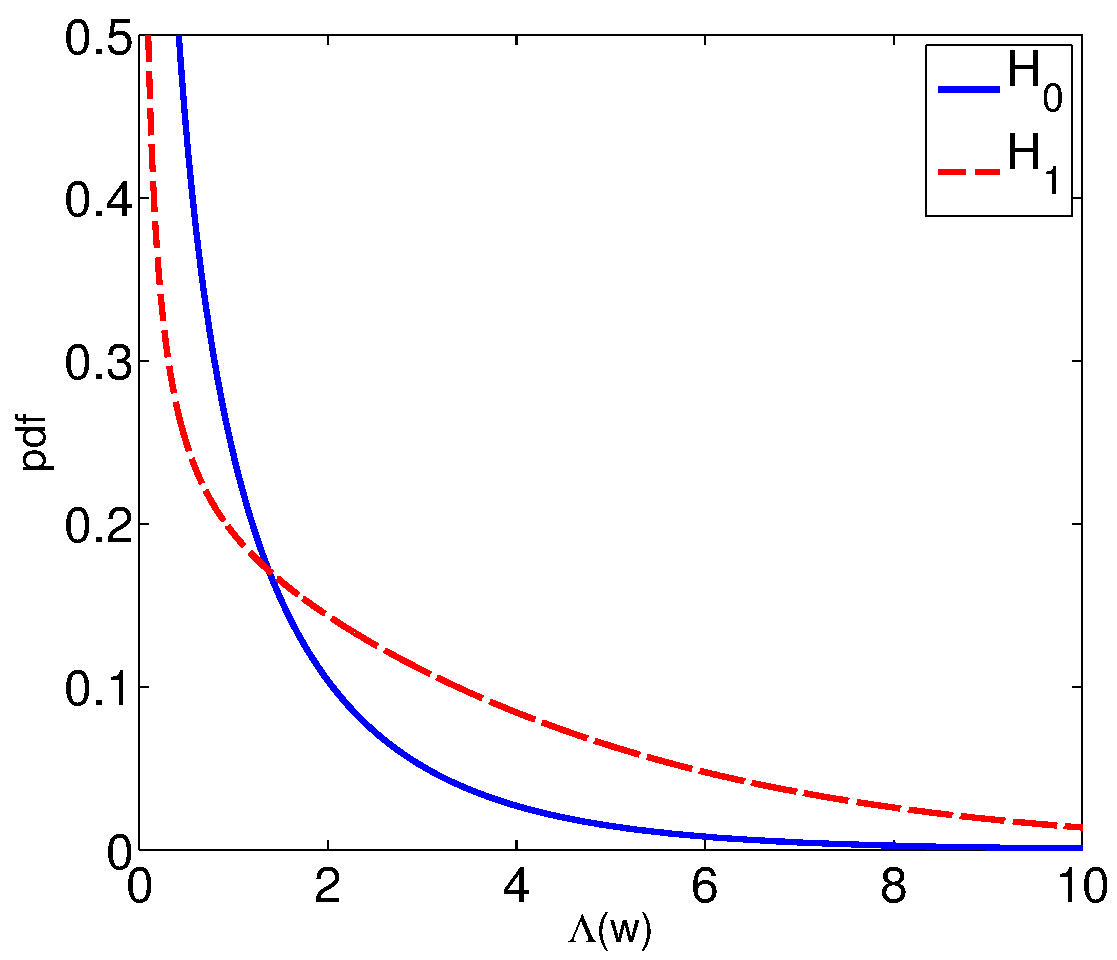
\includegraphics[width=0.3\textwidth]{taes_msd/figures/dist1.pdf}
  \label{fig:small}}
\subfigure[$d=2$, $\lambda_d=2$]{
  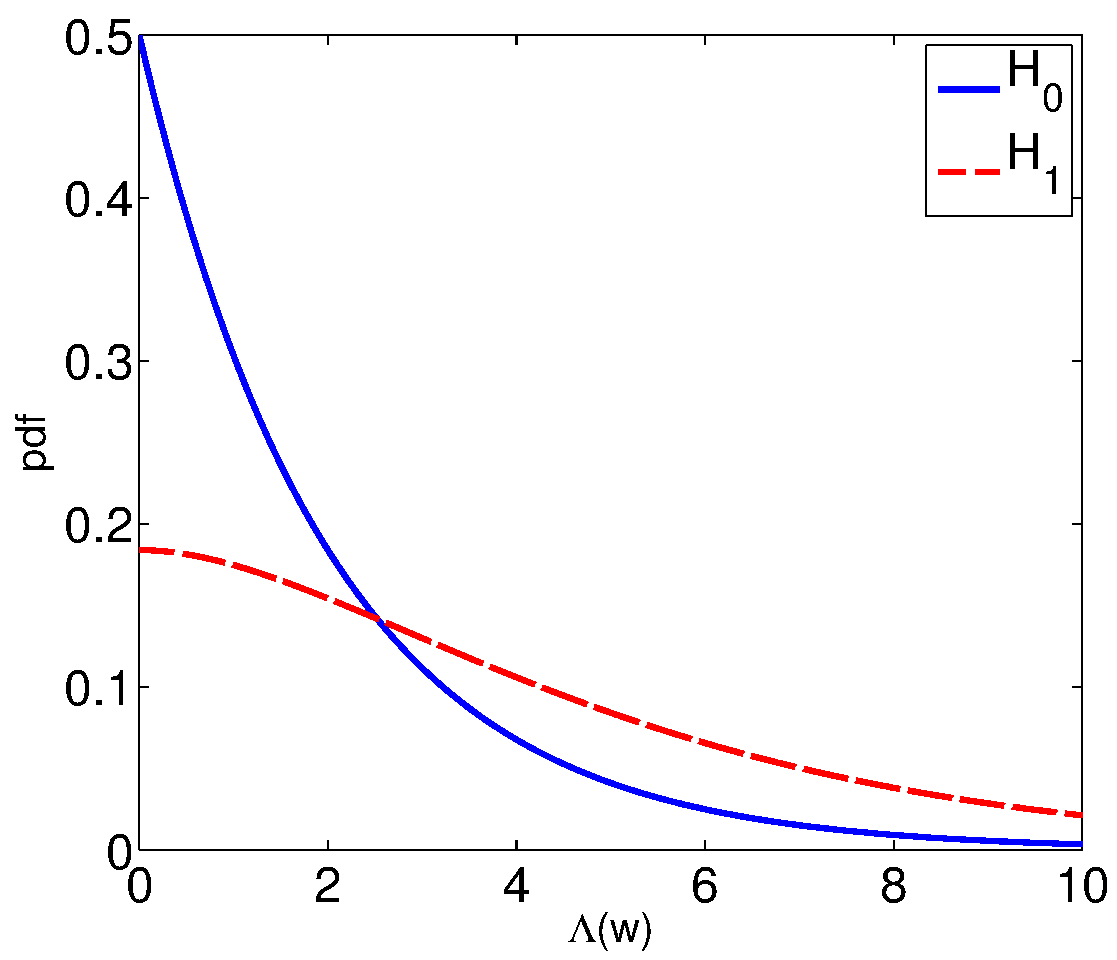
\includegraphics[width=0.3\textwidth]{taes_msd/figures/dist2.pdf}
  \label{fig:med}}
\subfigure[$d=2$, $\lambda_d=3$]{
  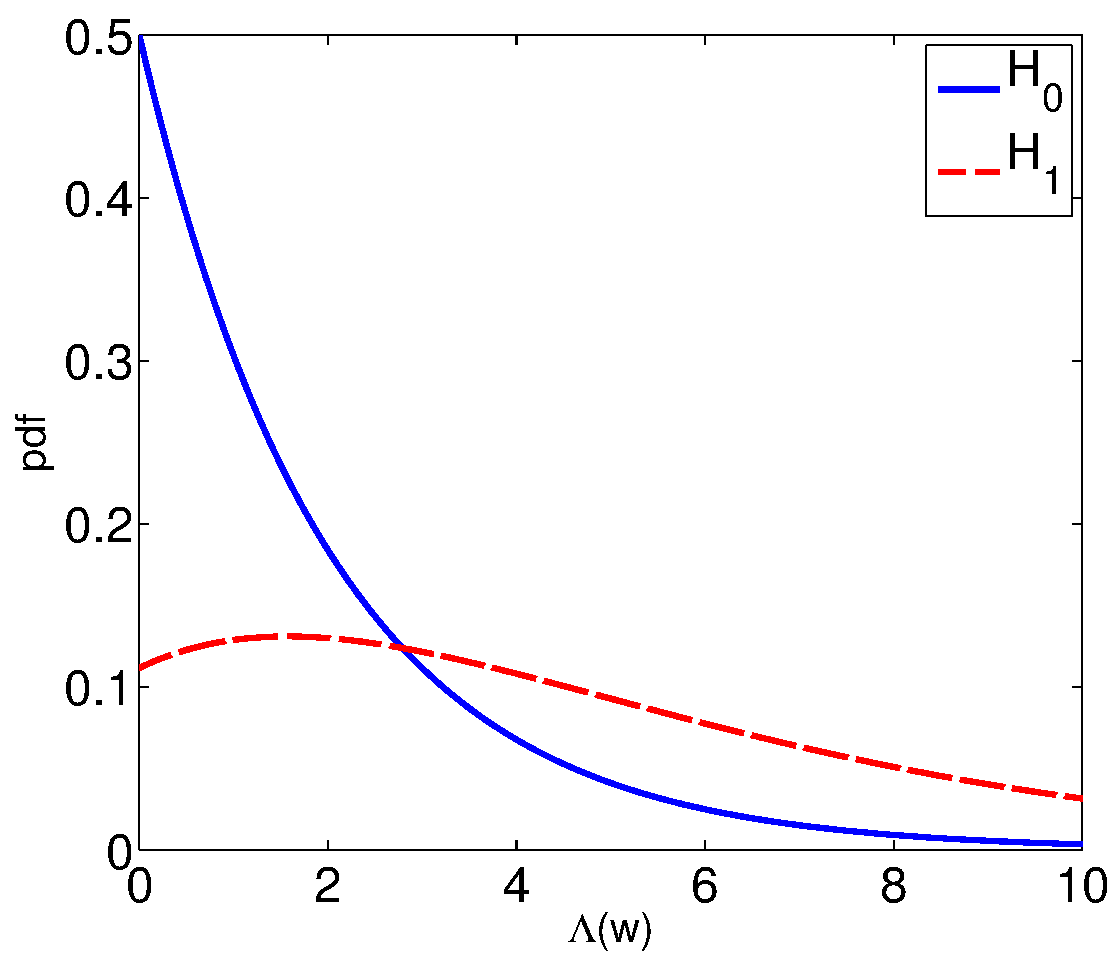
\includegraphics[width=0.3\textwidth]{taes_msd/figures/dist3.pdf}
  \label{fig:big}}
\caption{Probability density function (p.d.f.) of $\Lambda(w)\,|\,H_0$ and
  $\Lambda(w)\,|\,H_1$ for three combinations of the number of components $d$ and
  non-centrality parameter $\lambda_d$. (a) Baseline: $d=1$, $\lambda_d=2$ (b) Increases $d$
  but keeps $\lambda_d$ fixed. The distributions are less separable. (c) Increases both $d$
  and $\lambda_d$. The distributions are more separable.}
\label{fig:distributions}
\end{figure}

\begin{figure}[t]
  \centering
  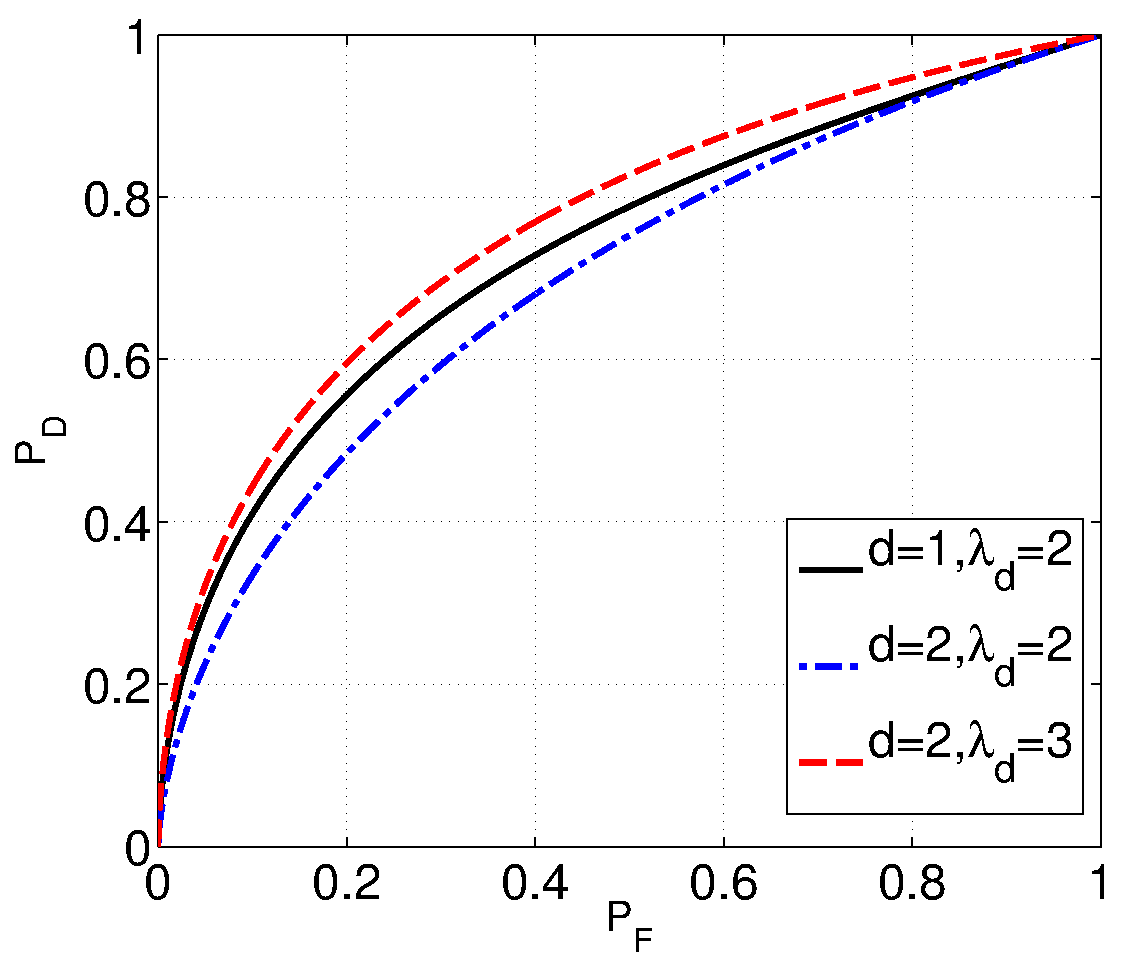
\includegraphics[width=\figwidth]{taes_msd/figures/dist_roc.pdf}
  \caption{The corresponding ROC curves to the three choices of $d$ and $\lambda_d$ in
    Figure \ref{fig:distributions}. ROC curves were generated from (\ref{eq:roc}). When
    adding an additional subspace component, the non-centrality parameter must increase
    sufficiently in order to achieve improved detection. }
  \label{fig:dist_roc}
\end{figure}

Finally, we explore the minimum increase in non-centrality parameter needed to improve
detection ability. Consider a setting with $d=1$ component and corresponding
non-centrality parameter $\lambda_1$. Let $\lambda_2$ be the resulting non-centrality
parameter by adding a second component, $d=2$, and let $\Delta\lambda=\lambda_2-\lambda_1$
be the resulting increase in non-centrality parameter. Figure \ref{fig:nc_lines} plots the
minimum increase in non-centrality parameter needed to improve detection as a function of
$\lambda_1$ for a few choices of $P_F$. If the increase in non-centrality parameter
exceeds this minimum threshold, that component is one of the $\kuse$ components.

We observe that the minimum increase in non-centrality parameter is dependent both on the
desired false alarm rate, $P_F$, and the first non-centrality parameter, $\lambda_1$.

The minimum increase in non-centrality parameter is larger for smaller false alarm rates
and is larger for larger $\lambda_1$. This is intuitive because larger values of
$\lambda_1$ separate the conditional distributions very well, indicating that the first
component is an excellent discriminant between the two hypotheses $H_0$ and $H_1$. For the
second component to improve detection ability, its contribution to the non-centrality
parameter must be larger for larger $\lambda_1$. Otherwise, the second component only adds
more noise to the detector. More generally, for the $i$th component to be one of the
$\kuse$ components, $\delta_i^2$ must exceed a critical threshold that is dependent on
$\sum_{j=1}^{i-1}\delta_j^2$. 

\begin{figure}[t]
\centering
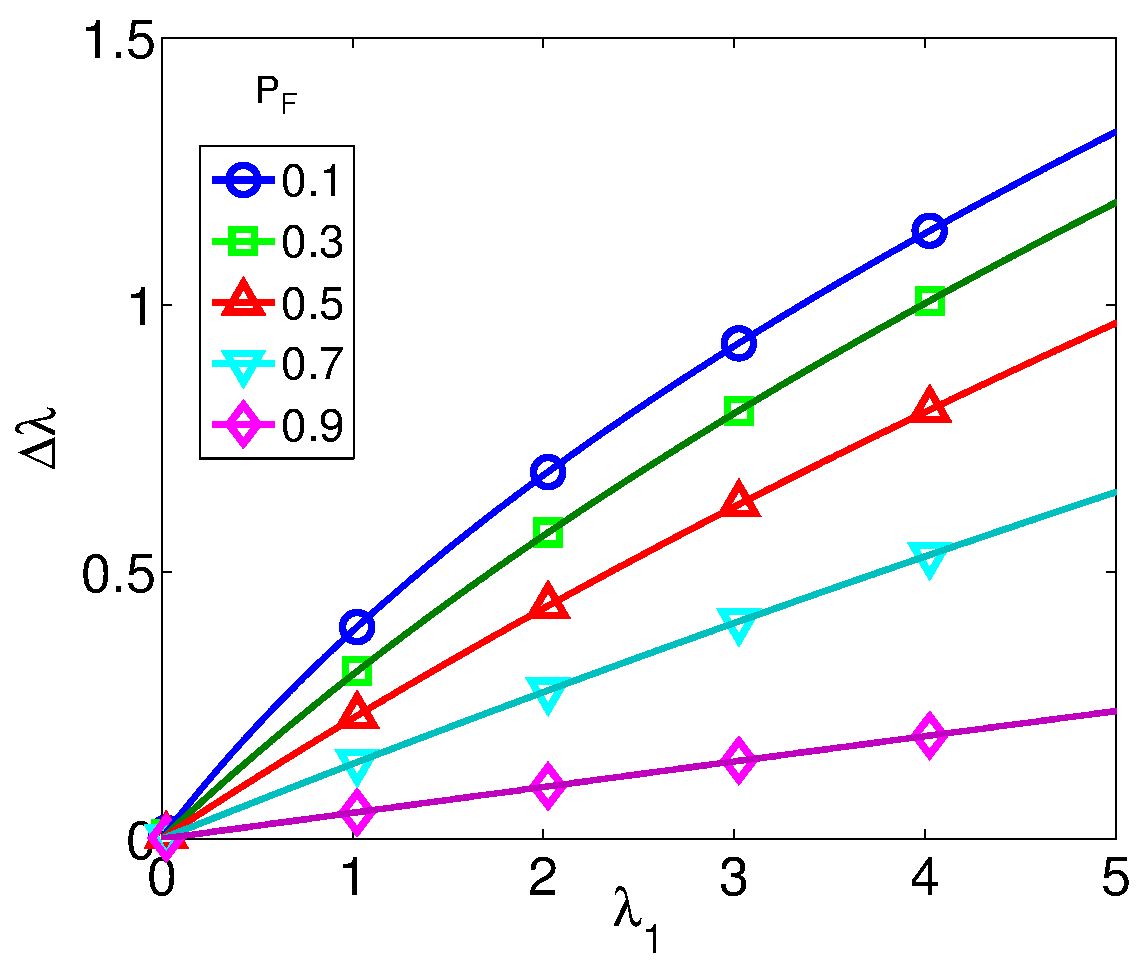
\includegraphics[width=\figwidth]{taes_msd/figures/nc_lines.pdf}
\caption{Minimum increase in non-centrality parameter necessary for increased detector
  performance. Results are shown for multiple choices of $P_F$. $\lambda_1$ indicates the
  non-centrality parameter when $d=1$ and $\Delta\lambda$ indicates the increase in
  non-centrality parameter when increasing the number of components to $d=2$.}
\label{fig:nc_lines}
\end{figure}
